\chapter{Results}

	In this chapter the results of GPU design choices and algorithmic optimizations
	and their effects are reviewed.

	\section{Software Shader Performance}

		The shader performed as expected, a conventional graphics card is 
		capable of rendering scenes with low scene complexity in real-time
		using sphere tracing.

		However scenes can easily be made to look a lot more complex than they 
		are, for example, by using mod fields or fractals. The hardware that 
		the shader was tested on (Geforce GTX 1060M) 20 reflective spheres could
		be rendered in real time in fullHD using our performance enhancing 
		algorithm.
		


	\section{GPU Performance}

		It is important to note that almost no effort was spent trying to
		optimize the performance of our design. 
	
	\section{Square roots}

		\begin{figure}[H]
			\centering
			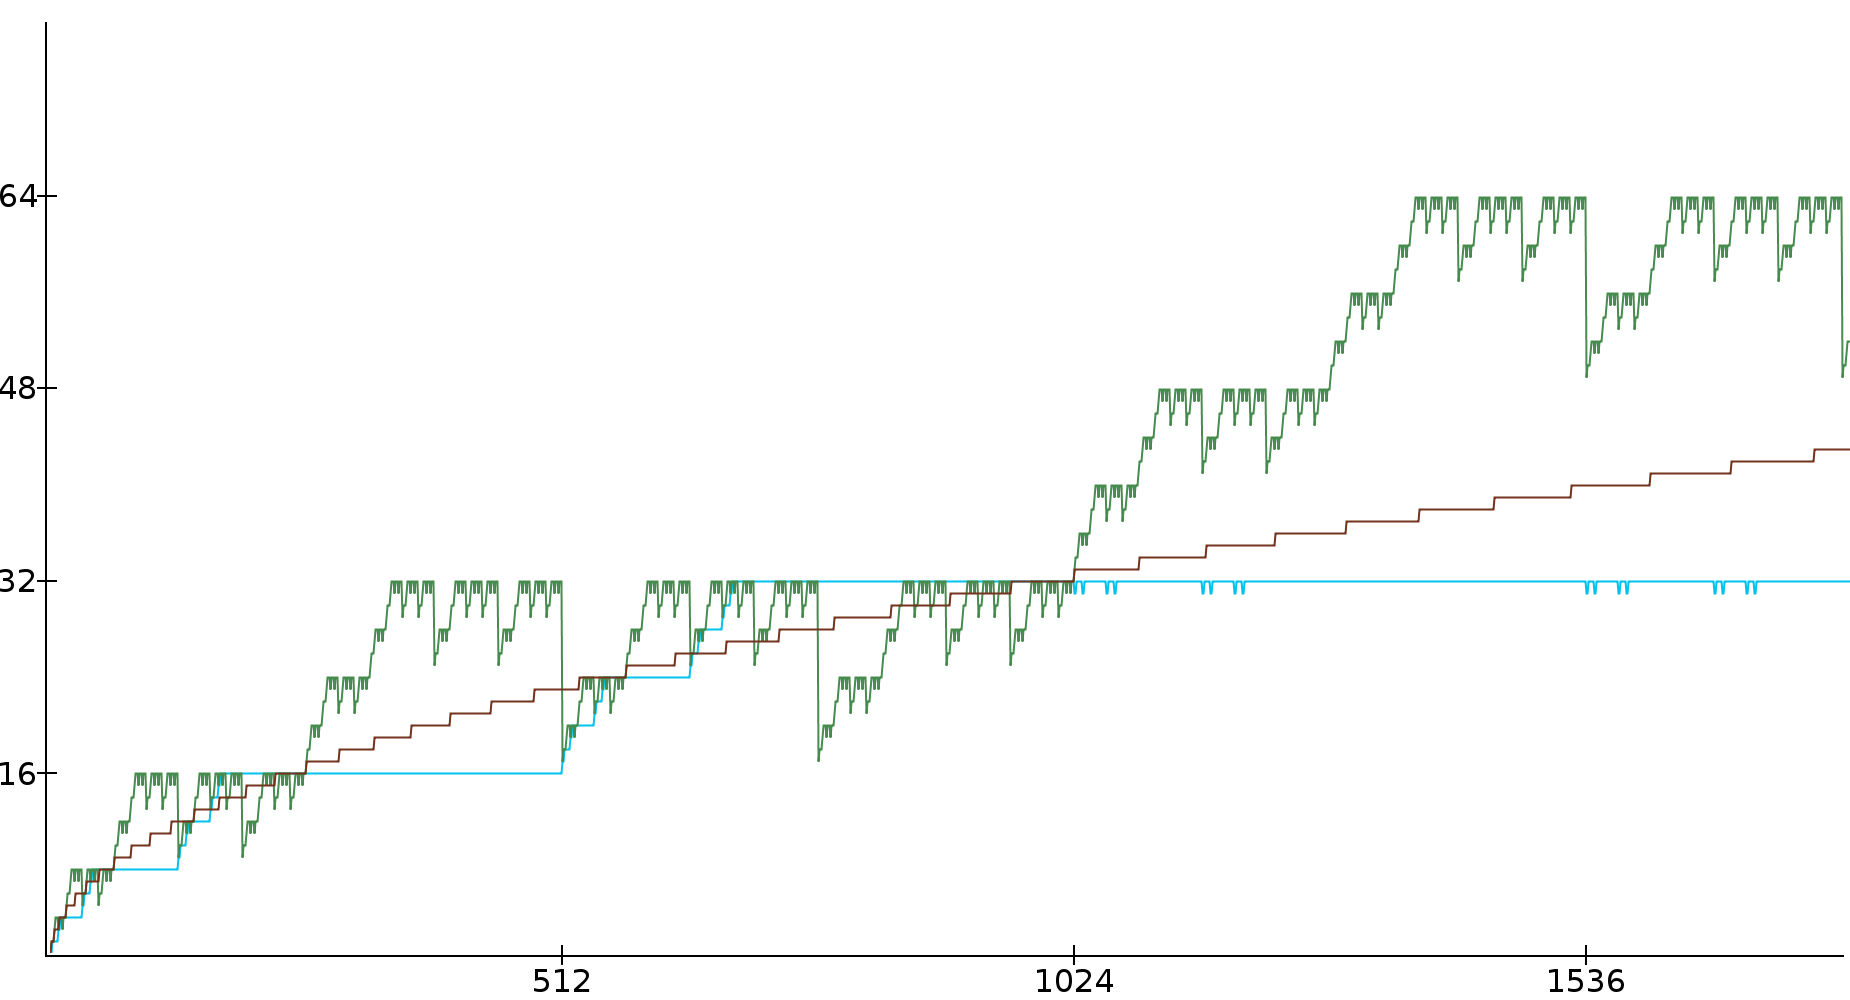
\includegraphics[width=0.75\linewidth]{figure/value12x.png} 
			\caption{Result from the simple square root approximator (green),
				the improved version (blue), and the shifting nth root 
				algorithm (red).}
			\label{orsqrt2}
		\end{figure}

		\begin{figure}[H]
			\centering
			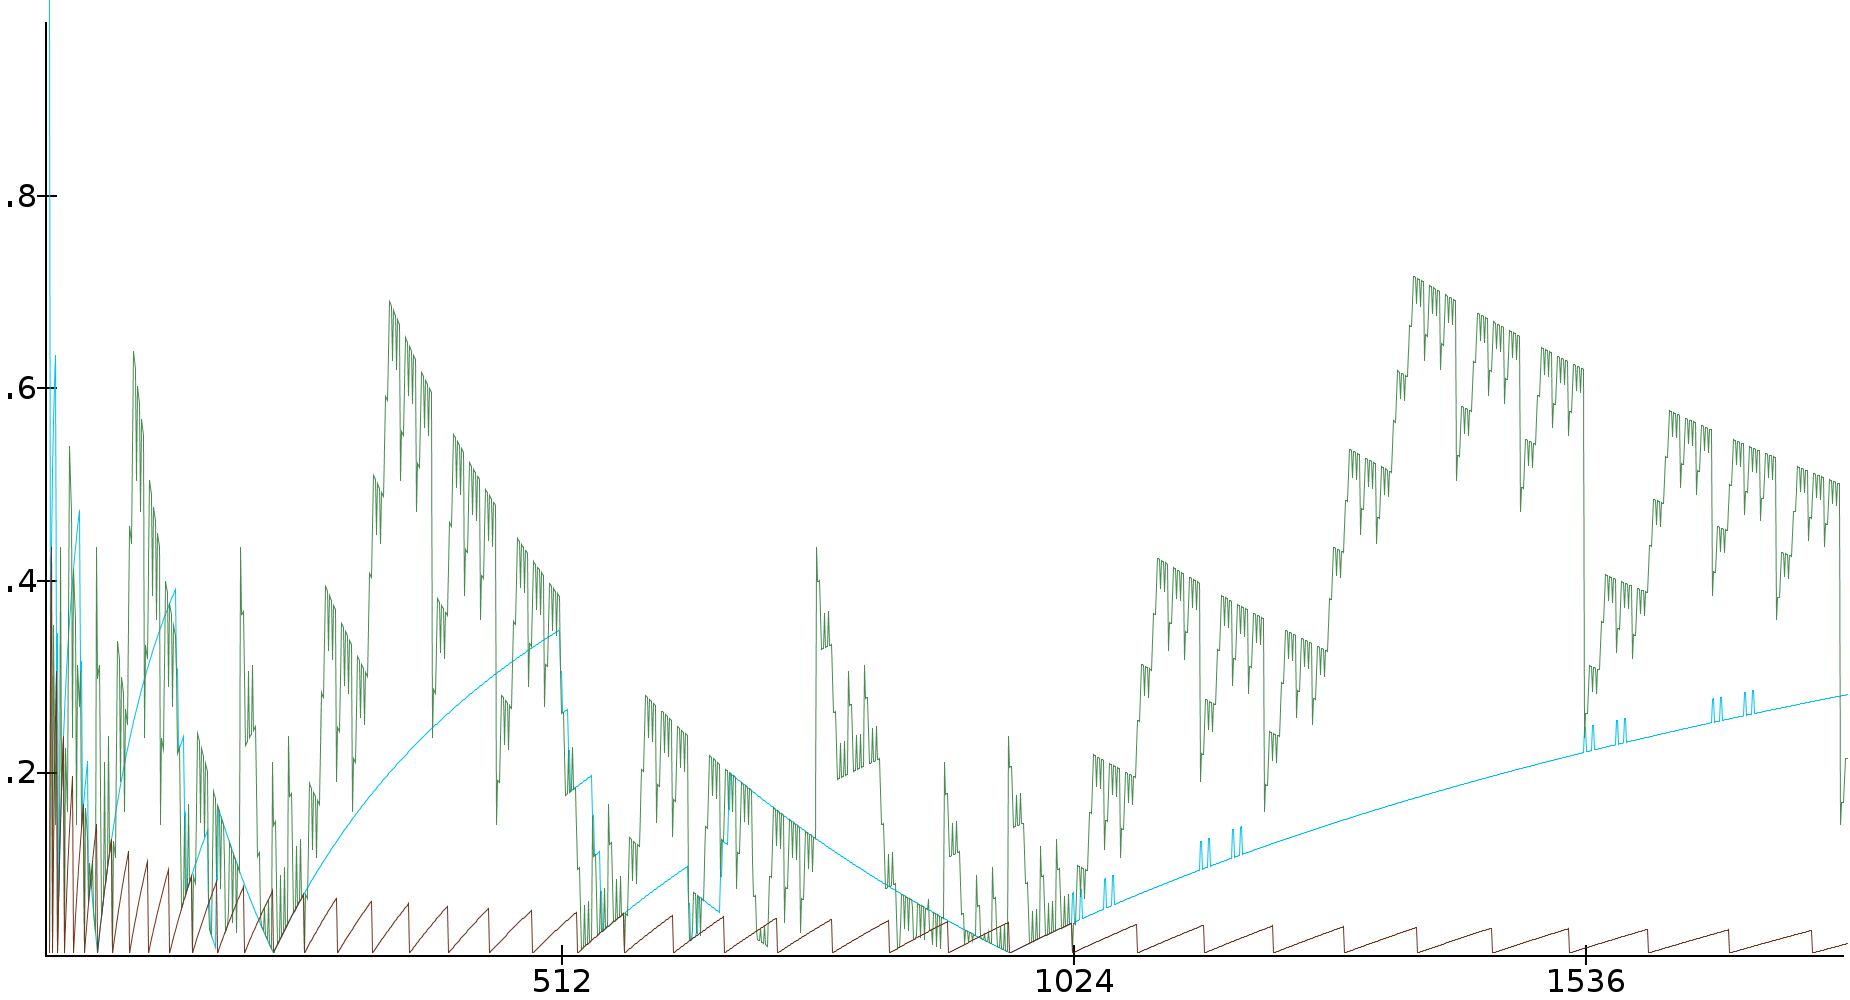
\includegraphics[width=0.75\linewidth]{figure/rel_error_480x.png} 
			\caption{Relative error for the simpe square root approximator
				(green), the improved version (blue), and the shifting nth root
				algorithm (red).}
			\label{orsqrt2}
		\end{figure}

		\begin{figure}[H]
			\centering
			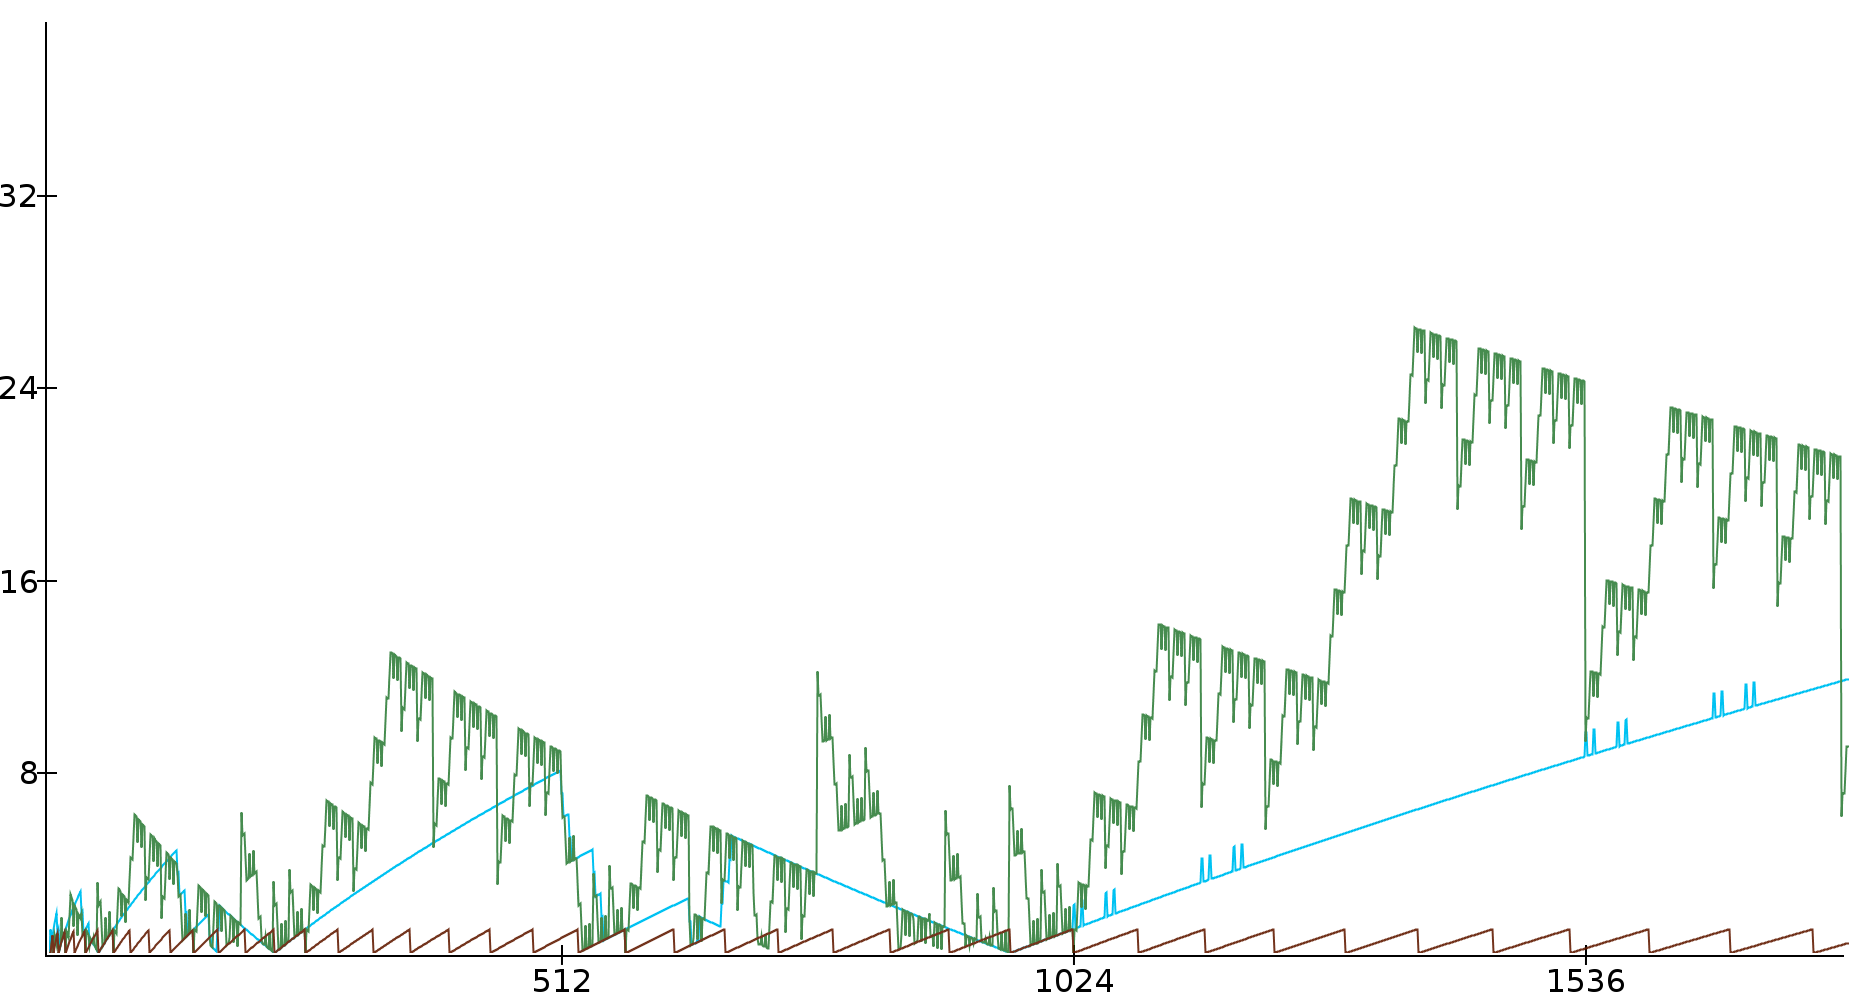
\includegraphics[width=0.75\linewidth]{figure/abs_error_24x.png} 
			\caption{Absolute error for the simpe square root approximator
				(green), the improved version (blue), and the shifting nth root
				algorithm (red).}
			\label{orsqrt2}
		\end{figure}

	\section{Optimizations}
		
		During this project, a number of optimizations were discussed and
		developed, the developed are explained here and the theoretical ones
		are brought up in the discussion section. Some of these are based on
		earlier work, with some others we believe are quite different from
		optimizations that have been discussed for sphere tracing previously.

		\subsection{Orthogonal culling}

			Orthogonal culling was implemented in the software shader and
			increased the performance.

			The test was performed such that we put an increasing number of
			solid-colored spheres in a plane in front of the camera. Because of
			this, the spheres are not obstructed by other spheres, making this
			the best possible scenario for the optimization.

			The test was set up such that we put an increasing number of
			solid-colored spheres in a plane in front of the camera. Because of
			this, the spheres are not obstructed by other spheres, making this
			the best possible scenario for the optimization.

			\begin{table}
			\centering
			\begin{tabular}{lll}
				\hline
				Objects & Optimized & Unoptimized \\ 
				\hline
				1       & 600       & 350         \\ 
				5       & 430       & 180         \\			
				10      & 290       & 98          \\
				15      & 85        & 13          \\
				20      & 58        & 9           \\
				25      & 40        & 6           \\
				30      & 29        & 4           \\
				35      & 7         & 3           \\
				40      & 6         & 2           \\
				45      & 4         & 1.5         \\
				\hline
			\end{tabular}
			\caption{Frames generated per second using the GLSL shader with and
				without the orthogonal culling optimization.}
			\end{table}

		\subsection{Bounding spheres}

			Bounding spheres was implemented and tested, there was a clear
			gain in performance but the results are depending on to many 
			factors to be able to review (number of objects, how dispersed the objects are, 
			size and place of the bounding sphere, etc.) . The larger the bounding sphere, the 
			less performance gain will be seen and the more objects that can 
			fit into a bounding sphere the more performance gain will be seen.
			This optimization could be used to decrease the performance too, by
			setting up a too large boundnig sphere or my setting it up with few
			objects that are far apart.

			To use this optimiztion efficiently the objects inside a bounding 
			sphere should never come far apart and the sphere should be defined
			to never be exactly the right size. 
